\documentclass[12pt,a4paper]{article}
\usepackage[utf8]{inputenc}
\usepackage{geometry}
\usepackage{graphicx}
\usepackage{booktabs}
\usepackage{hyperref}
\usepackage{float}

\geometry{margin=2.5cm}

\title{Diabetes Dataset Analysis Report}
\author{Nadir NEHILI}
\date{\today}

\begin{document}

\maketitle

\section{Introduction}
This report presents an exploratory analysis of the \textbf{Diabetes dataset} from Kaggle. The dataset contains 768 observations and 9 variables, with the goal of investigating factors related to type 2 diabetes occurrence.

\section{Dataset Overview}
The dataset includes the following columns:

\begin{itemize}
    \item \textbf{Pregnancies} : Number of times pregnant
    \item \textbf{Glucose} : Plasma glucose concentration
    \item \textbf{BloodPressure} : Diastolic blood pressure (mm Hg)
    \item \textbf{SkinThickness} : Triceps skinfold thickness (mm)
    \item \textbf{Insulin} : 2-Hour serum insulin (mu U/ml)
    \item \textbf{BMI} : Body mass index (weight in kg/(height in m)$^2$)
    \item \textbf{DiabetesPedigreeFunction} : Diabetes pedigree function
    \item \textbf{Age} : Age in years
    \item \textbf{Outcome} : Target variable (0 = Non-Diabetic, 1 = Diabetic)
\end{itemize}

\section{Missing / Invalid Values Before Cleaning}
Some columns contain physically impossible zero values, which should be treated as missing for analysis. The counts of missing or invalid values are presented in Table~\ref{tab:missing_values}.

\begin{table}[H]
\centering
\begin{tabular}{lr}
    \toprule
    \textbf{Column} & \textbf{Missing / Invalid Values} \\
    \midrule
    Pregnancies & 0 \\
    Glucose & 5 \\
    BloodPressure & 35 \\
    SkinThickness & 227 \\
    Insulin & 374 \\
    BMI & 11 \\
    DiabetesPedigreeFunction & 0 \\
    Age & 0 \\
    Outcome & 0 \\
    \bottomrule
    \end{tabular}
    
\caption{Number of missing or invalid values per column before cleaning.}
\label{tab:missing_values}
\end{table}

\section{Data Cleaning Method}
To handle invalid values, all zeros in the affected columns (\texttt{Glucose}, \texttt{BloodPressure}, \texttt{SkinThickness}, \texttt{Insulin}, \texttt{BMI}) were replaced with the \textbf{median} of the respective column. This preserves the distribution of the data while correcting unrealistic entries.

After cleaning, the dataset contains no zeros in the previously affected columns, as summarized in Table~\ref{tab:after_cleaning}.

\begin{table}[H]
\centering
\begin{tabular}{lr}
\toprule
\textbf{Column} & \textbf{Zero Values Remaining} \\
\midrule
Glucose & 0 \\
BloodPressure & 0 \\
SkinThickness & 0 \\
Insulin & 0 \\
BMI & 0 \\
\bottomrule
\end{tabular}
\caption{Number of zero values remaining after cleaning.}
\label{tab:after_cleaning}
\end{table}

The cleaned dataset has been exported as \texttt{data/diabetes\_cleaned.csv} for further analysis.

\section{Exploratory Data Analysis}

\subsection{Boxplots by Outcome}

\begin{figure}[H]
\centering
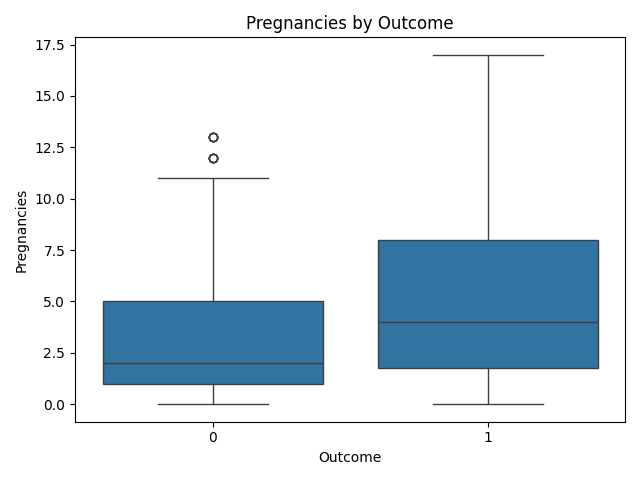
\includegraphics[width=0.8\textwidth]{../plots/boxplot_Pregnancies.png}
\caption{Pregnancies by Outcome}
\end{figure}

\begin{figure}[H]
\centering
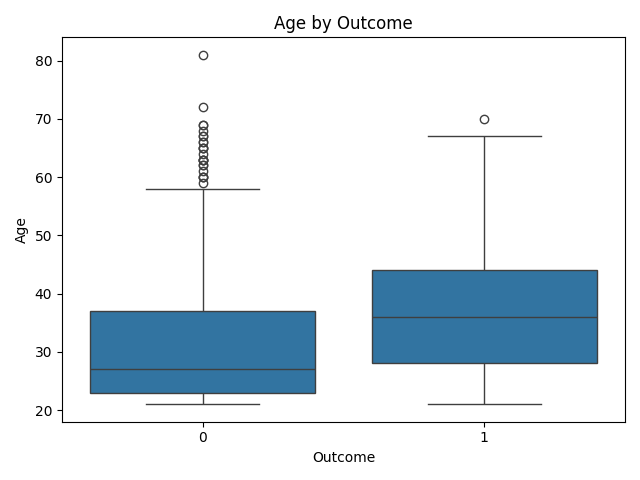
\includegraphics[width=0.8\textwidth]{../plots/boxplot_Age.png}
\caption{Age by Outcome}
\end{figure}

\begin{figure}[H]
\centering
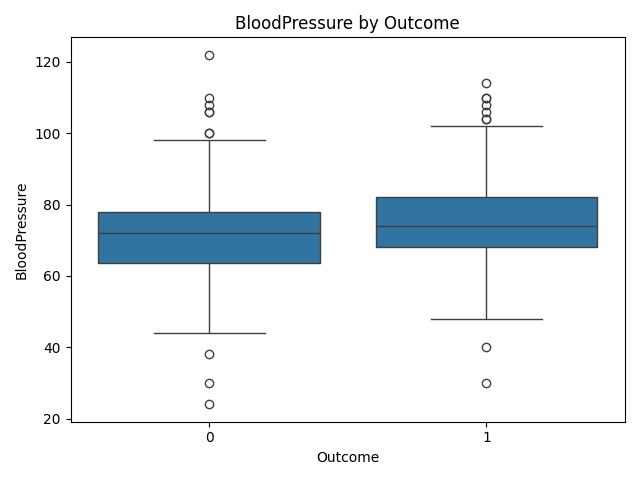
\includegraphics[width=0.8\textwidth]{../plots/boxplot_BloodPressure.png}
\caption{Blood Pressure by Outcome}
\end{figure}

\begin{figure}[H]
\centering
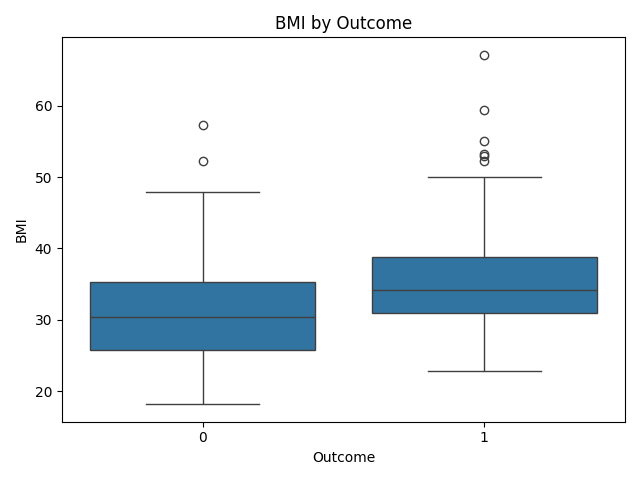
\includegraphics[width=0.8\textwidth]{../plots/boxplot_BMI.png}
\caption{BMI by Outcome}
\end{figure}

\begin{figure}[H]
\centering
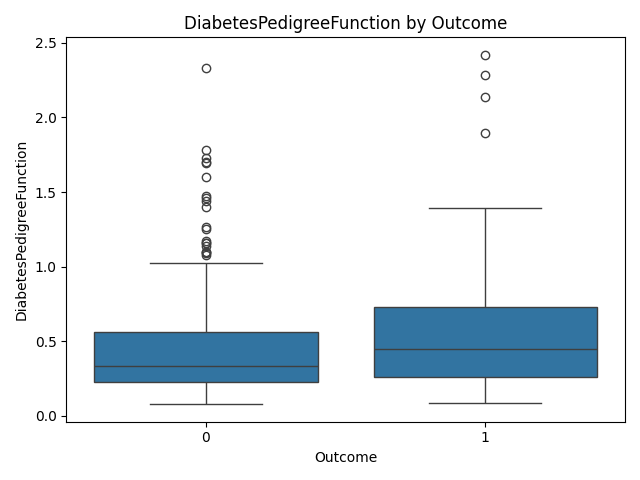
\includegraphics[width=0.8\textwidth]{../plots/boxplot_DiabetesPedigreeFunction.png}
\caption{Diabetes Pedigree Function by Outcome}
\end{figure}

\begin{figure}[H]
\centering
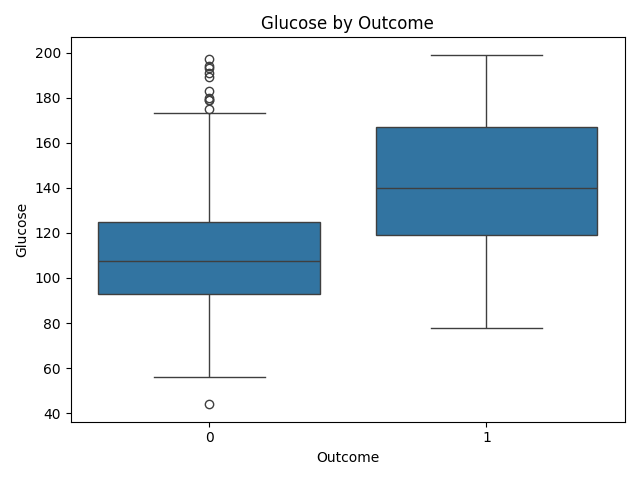
\includegraphics[width=0.8\textwidth]{../plots/boxplot_Glucose.png}
\caption{Glucose by Outcome}
\end{figure}

\begin{figure}[H]
\centering
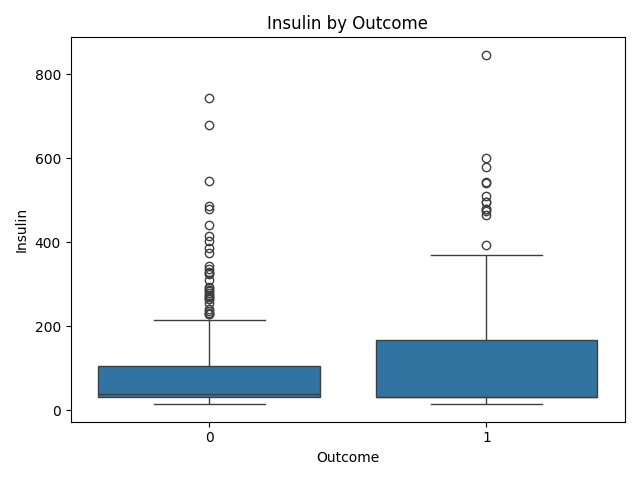
\includegraphics[width=0.8\textwidth]{../plots/boxplot_Insulin.png}
\caption{Insulin by Outcome}
\end{figure}

\begin{figure}[H]
\centering
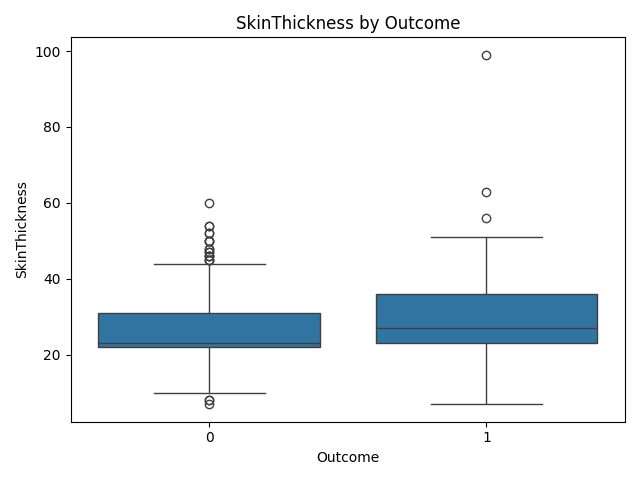
\includegraphics[width=0.8\textwidth]{../plots/boxplot_SkinThickness.png}
\caption{Skin Thickness by Outcome}
\end{figure}

\subsection{Correlation Heatmap}
\begin{figure}[H]
\centering
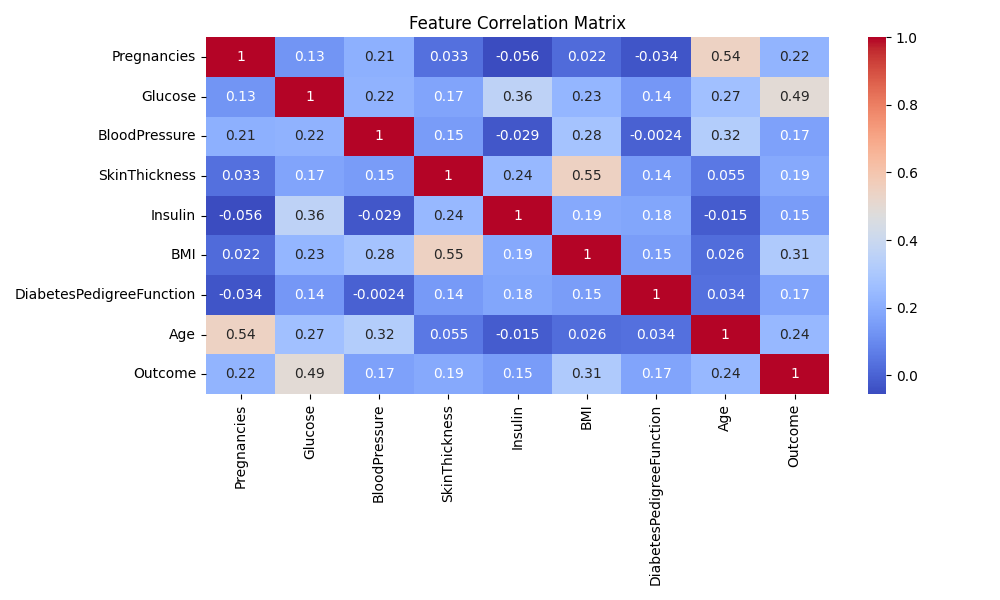
\includegraphics[width=0.9\textwidth]{../plots/correlation_heatmap.png}
\caption{Correlation matrix of features}
\end{figure}



\subsection{Detailed Analysis of Plots}
Based on the provided box plots and correlation heatmap, here is a detailed analysis of the factors associated with diabetes.

\subsubsection{Box Plots Analysis}
\textbf{Glucose}: This variable shows the clearest distinction between the two groups. The median and the entire interquartile range (IQR) for diabetic individuals (Outcome 1) are significantly higher than for non-diabetics (Outcome 0). This strongly suggests that high glucose levels are a key indicator of diabetes.

\textbf{Age}: The median age of the diabetic group (1) is higher. This group also shows a wider spread of ages, indicating that diabetes affects an older population on average.

\textbf{BMI}: The diabetic group (1) has a higher median BMI and a generally higher distribution of values than the non-diabetic group (0). This points to a strong link between a higher BMI and the presence of diabetes.

\textbf{DiabetesPedigreeFunction}: The median and distribution of this function are higher for diabetic individuals (1). This suggests that a family history of diabetes, as measured by this function, is a significant risk factor.

\textbf{Pregnancies}: The median and spread of pregnancies are higher in the diabetic group (1). This could indicate that the number of pregnancies is a factor associated with diabetes.

\textbf{Insulin}: The medians of both groups are very similar. However, the distribution is wider for diabetics (1), and both groups show a large number of outliers, especially the non-diabetic group (0). Insulin alone does not seem to be as clear an indicator as glucose.

\textbf{BloodPressure}: The medians of both groups are very close, and the distributions overlap considerably. This suggests that blood pressure, as a single variable, is not a very distinctive factor for predicting diabetes in this dataset.

\textbf{SkinThickness}: The median for diabetics (1) is slightly higher, but the difference is not as pronounced as for glucose or BMI. The distributions of the two groups are quite similar.

\subsubsection{Correlation Heatmap Analysis}
By examining the "Outcome" row/column, we can see the correlation of each variable with the presence of diabetes:

\textbf{Strong Correlation}:
\textbf{Glucose}: The highest correlation (0.49). This confirms what was observed in the box plot: glucose levels are the factor most strongly linked to diabetes.

\textbf{BMI}: Moderate correlation (0.31).

\textbf{Age}: Moderate correlation (0.24).

\textbf{Weak to Moderate Correlation}:
\textbf{Pregnancies}: Correlation of 0.22.

\textbf{SkinThickness}: Correlation of 0.19.

\textbf{DiabetesPedigreeFunction}: Correlation of 0.17.

\textbf{Weak Correlation}:
\textbf{BloodPressure}: The correlation is very weak (0.17), which confirms the observation from the box plot.

\textbf{Insulin}: The correlation is also very weak (0.15).

\section{Conclusion}
The initial analysis identified missing or invalid values in several columns, which were cleaned by replacing zeros with the median. The EDA plots provide an overview of feature distributions, correlations, and differences between diabetic and non-diabetic individuals.

Based on this exploratory data analysis, we can conclude that Glucose levels are the most significant factor associated with diabetes, followed by BMI and Age. Other variables such as \textbf{Pregnancies} and the \textbf{DiabetesPedigreeFunction} also show a notable association. \textbf{Blood Pressure} and Insulin appear to be the least correlated with the outcome in this dataset. The cleaned dataset is now ready for more advanced analysis, including predictive modeling, using these key variables as primary predictors.

\end{document}
